\subsubsection{Cost Function}
\begin{itemize}[--]
	\item Suppose we have:
	\begin{itemize}[--]
		\item Training sets: $\left\{ (x^{(1)}, y^{(1)}),\ldots, (x^{(m)}, y^{(m)})  \right\}$
		\item $m=$ number of training examples
		\item $L=$ total number of layers in network
		\item $s_l=$ number of units (not counting bias unit) in layer $l$
		\item $k=$ number of classes
	\end{itemize}

	\item Binary Classification:
	\begin{itemize}[--]
		\item $y=0\text{ or } 1$
		\item 1 output unit $h(x)\in\mathbb{R}$
		\item $s_l=1$
		\item $k=1$
	\end{itemize}

	\item Multi-class Classification ($K$ classes)
	\begin{itemize}[--]
		\item $y\in\mathbb{R}^K$
		\item $K$ output units
		\item $h(x)\in\mathbb{R}^K$
		\item $s_l=K, (K\geq 3)$
	\end{itemize}

	\item New cost function:
		$$h_{\Theta}(x)\in\mathbb{R}^K, (h_{\Theta}(x))_i=i^{\text{th}}\text{ output}$$
		$$J(\Theta)=-\frac{1}{m}\left[
			\sum_{i=1}^{m}\sum_{k=1}^{K} y_k^{(i)}\log (h(x^{(i)}))_k + (1-y_k^{(i)})\log (1- h(x^{(i)})_k)
			\right] + \frac{\lambda}{2m}\sum_{l=1}^{L-1}\sum_{i=1}^{s_l}\sum_{j=1}^{s_l + 1} (\Theta_{ji}^{(l)})^2$$
\end{itemize}

\subsubsection{Backpropagation Algorithm}
\begin{itemize}[--]
	\item In order to perform gradient descent we need to compute $J(\Theta), \frac{\partial}{\partial\Theta_{ij}}^{(l)} J(\Theta)$
	\item We have already defined $J(\Theta)$, so we just need the partial derivatives.
	\item Intuition: $\delta_j^{(l)}=$ ``error'' of node $j$ in layer $l$
	\item An example is for each output unit (layer $L=4$): $\delta_{j}^{(4)}=a_{j}^{(4)} - y_{j}$
	\item We will comput the $\delta$ for every layer of the neural network
		$$\delta^{(n)} = (\Theta^{(3)})^{T}\delta^{(n+1)} .\times g'(z^{(n)})$$
	\item Where $.\times$ is element-wise multiplication
	\item There is no erro associated with the input layer
	\item The name backpropagation, comes from calculating the error from the back towards the beginning of the network

	\item Suppose we have a training set of $m$ examples
	\item We will set $\Delta_{ij}^{(l)}=0$ (for all $l,i,j$)
	\item This will be used to compute the partial derivatives of the cost function

	TODO: turn into pseudocode

	For $i=1$ to $m$:
		Set $a^{(1)}=x^{(i)}$
		Perform forward propagation to compute $a^{(l)}$ for $l=2,3,\ldots, L$
		Using $y^{(i)}$, comput $\delta^{(L)}=a^{(L)}-y^{(i)}$
		Compute $\delta^{(L-1)}, \delta^{(L-2)}, \ldots, \delta^{(2)}$
		$\Delta_{ij}^{(l)}:=\Delta_{ij}^{(l)} + a_j^{(l)} \delta_i^{(l+1)}$

	\item It's possible to vectorize the final update: $\Delta^{(l)} := \Delta^{(l)} + \delta^{(l+1)} (a^{(l)})^{T}$
	\item After completing the loop we calculate:
		$$D_{ij}^{(l)} := \frac{1}{m}\Delta_{ij}^{(l)} + \lambda\Theta_{ij}^{(l)} \text{ if } j\neq 0$$
		$$D_{ij}^{(l)} := \frac{1}{m}\Delta_{ij}^{(l)} \text{ if } j=0$$
		$$\frac{\partial}{\partial\Theta_{ij}^{(l)}} J(\Theta) = D_{ij}^{(l)}$$
\end{itemize}

\subsubsection{Backpropagation Intuition}
\begin{itemize}[--]
	\item Let us first take another look at forward propagation
	\item We first feed an input into the input layer $x^{(i)}$, then we calculate the second layer $z_1^{(2)}\to a_1^{(2)}$, similarly for the next 2 layers
	\begin{center}
		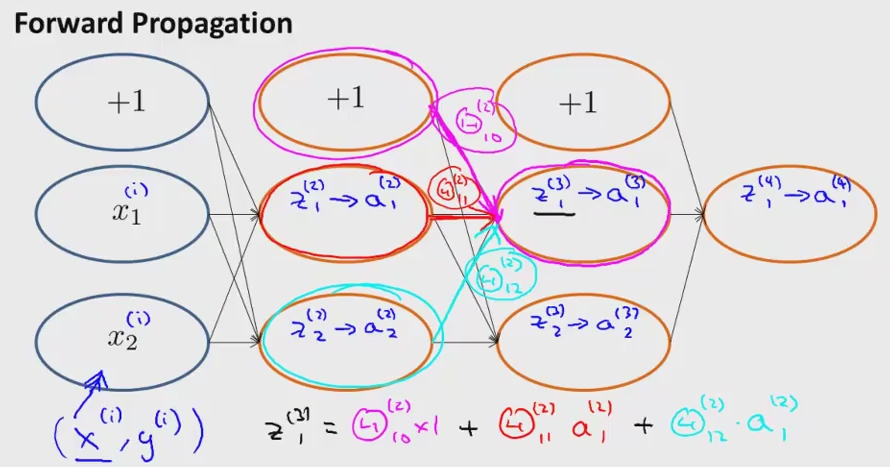
\includegraphics[scale=0.7]{sections/cs229/w6/forward_prop.png}
	\end{center}

	\item If you focus on a single example, the case of 1 output unit, and ignoring regularization ($\lambda = 0$): 
		$$\text{cost}(i)=y^{(i)}\log h(x^{(i)}) + (1-y{(i)} ) \log h(x^{(i)} )$$
	\item Formally, $\delta_j^{(l)}=\frac{\partial}{\partial z_j^{(l)}}\text{cost}(i)\text{ for } j\geq 0$
	\item Backpropagation looks identical, but backwards:
	\begin{center}
		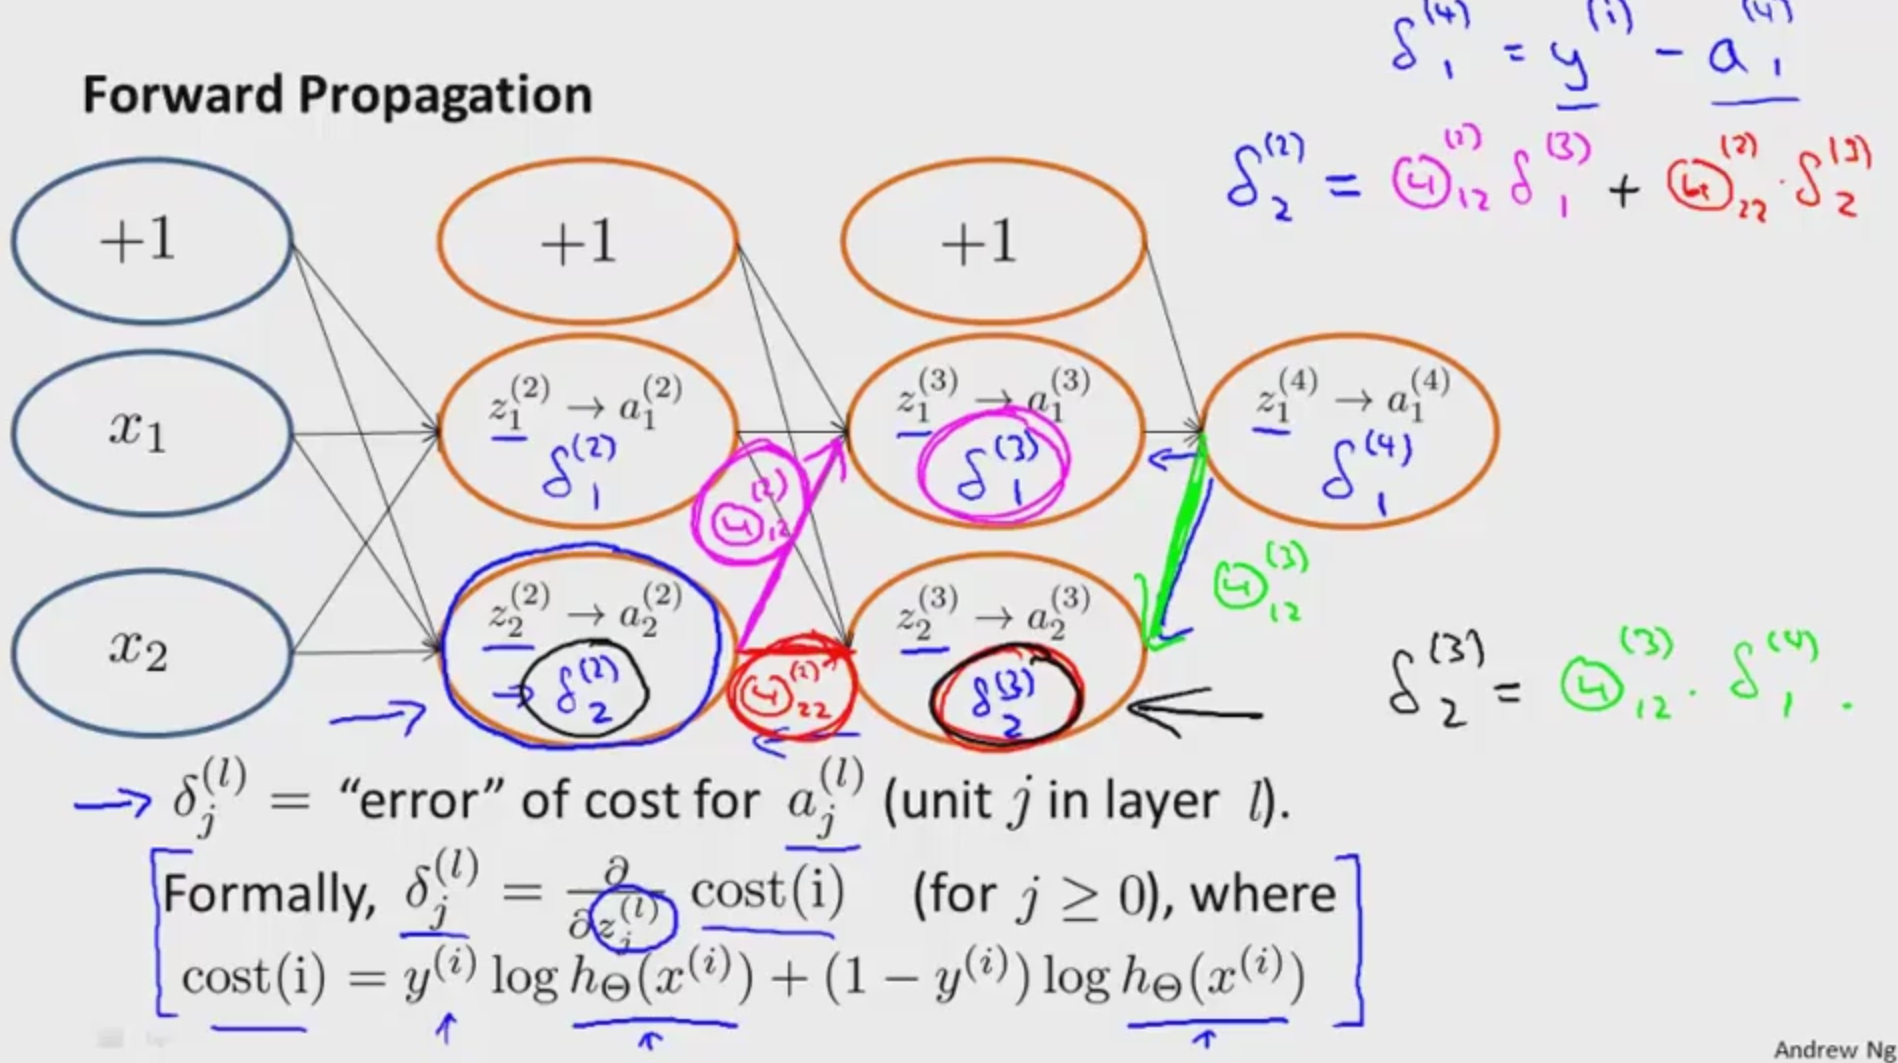
\includegraphics[scale=0.25]{sections/cs229/w6/back_prop.png}
	\end{center}
\end{itemize}

\subsubsection{Implementation Note: Unrolling Parameters}
\begin{itemize}[--]
	\item Our previous use of minfunc and costFunction in octave assumed that $\theta$ and the return would be vectors
	\item You can unroll elements into  large vector:
		thetaVec = [Theta1(:); Theta2(:); Theta3(:)];
	\item You can also change them back into the matrix using reshape:
		Theta1 = reshape(thetaVec(1:size),dim1, dim2);
	\begin{center}
		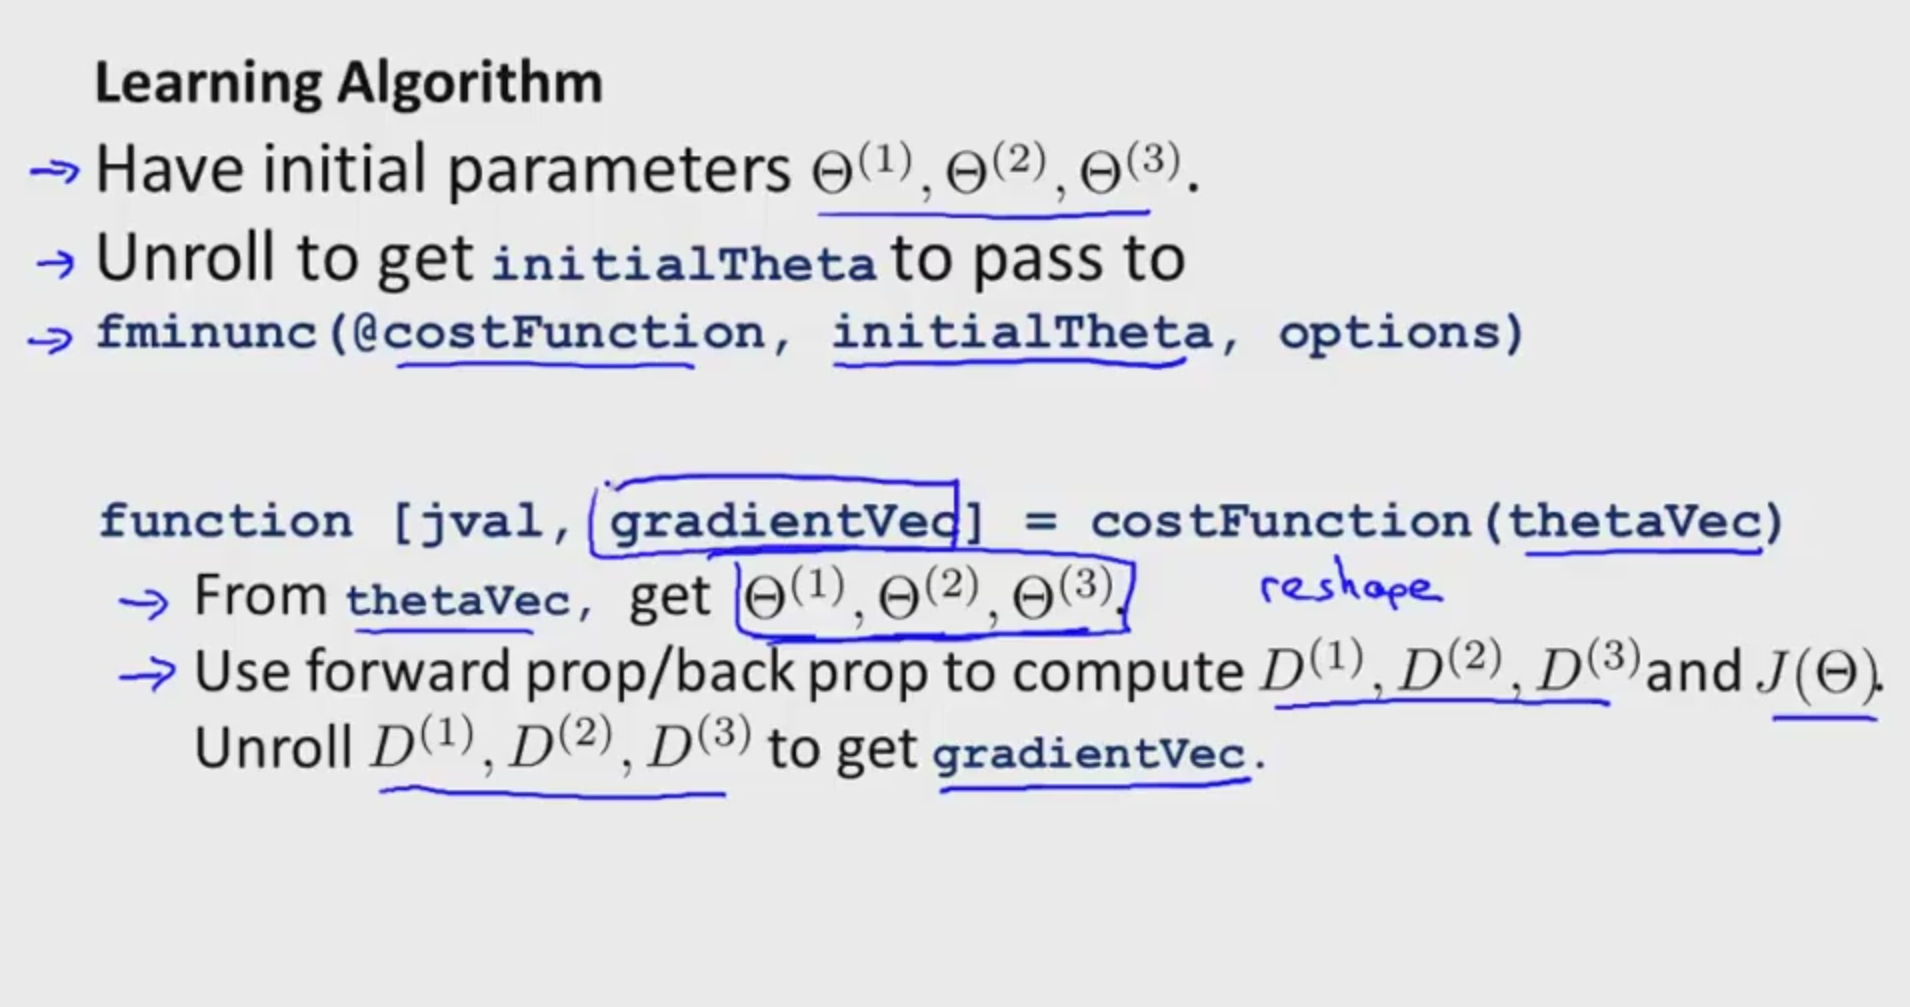
\includegraphics[scale=0.2]{sections/cs229/w6/algo.png}
	\end{center}
\end{itemize}

\subsubsection{Gradient Checking}
\begin{itemize}[--]
	\item Suppose you have a function $J(\Theta)$, and we want to estimate the derivative at $\theta\in\mathbb{R}$.
	\item We consider the points $\theta - \epsilon$ and $\theta + \epsilon$, and draw a line through these points and use the slope of this line as an approximation
	\item This gives our approximation as:
		$$\frac{d}{d\Theta} J(\Theta) = \frac{J(\Theta + \epsilon) - J(\Theta - \epsilon)}{2\epsilon}$$
	\item A good value for epsilon is: $\epsilon= 10^{-4}$
	\item Now consider $\theta\in\mathbb{R}^{n}$
	\item We can calculate the derivative for each element the same as we did for the single variable. Holding the other variables constant
	\item We then can compare this approximate derivative to the backpropagation to check that they're approximately the same
	\item Don't do gradient checking once you start learning, because it will be very slow
	\item j
\end{itemize}

\subsubsection{Random Initialization}
\begin{itemize}[--]
	\item Initializing all the parameters in a neural network, does not work like it did in our previous algorithms
	\item After each update, parameters corresponding to inputs going into each of two hidden units are identical
	\item This results in not being able to develop more complex features
	\item Instead, we will now initialize each $\Theta_{ij}^{(l)}$ to a random value in $\left[ -\epsilon, \epsilon \right]$
	\item The goal is ``symmetry breaking''
\end{itemize}

\subsubsection{Putting it Together}
\begin{itemize}[--]
	\item We must pick a network architecture (connectivity pattern between neurons)
	\item Reasonable default: 1 hidden layer, or if >1 hidden layer, have same number of hidden units in every layer (usually the more the better)
	\item Training a neural network:
	\begin{itemize}[--]
		\item Randomly initialize weights
		\item Implement forward propagation to get $h_{\Theta} (x^{(i)})$ for any $x^{(i)}$
		\item Impelement code to cmpute cost function $J(\Theta)$
		\item Implement backprop to compute partial derivatives $\frac{\partial}{\partial \Theta_{jk}^{(l)}} J(\Theta)$
		\item Perform forward propagation and backpropagation using each example
		\item Use gradient checking to compare partial derivatives computed using backpropagation vs. using numerical estimate of gradient of $J$. Then disable gradient checking code.
		\item Use gradient descent or advanced optimization method with backpropagation to try and minimize $J$ as a function of parameters $\Theta$
	\end{itemize}

	\item $J(\Theta )$ is non-convex, and can get stuck in local optimum
	
\end{itemize}